\documentclass[11]{article}

\usepackage{graphicx}
\usepackage{hyperref}
\usepackage{subcaption}
\usepackage{amsmath}
\usepackage[
    backend=bibtex,
%    isbn=false,
%    url=false,
%    doi=false,
%    eprint=false,
%    hyperref=false,
%    backref=false,
%    firstinits=false,
]{biblatex}
\bibliography{references}

\hypersetup{colorlinks,urlcolor=blue}
\let \shorttitle \textbf
\begin{document}

\section{Introduction}
Tool use is one of the abilities that uniquely distinguishes man from other species. 
We refer to tools as hand held devices employed in making changes to the surrounding environment. 
Cases of tool use have been reported in other species, but never to the extent engaged by humans \cite{boysen1999,harrington2009,lefebvre2004}. 
As a defining attribute of human cognition, we wish to lay the foundations for a computational model of tool use reasoning.

Our model stems from the architectural framework defined by the four constraints theory (4CT) \cite{osiurak2014a}.
In the following we describe 4CT and its implications to the project.  

\subsection{The Four Constraints Theory}
4CT defines tool use behaviour of healthy individuals based on empirical investigations of apraxia.
Apraxia is a neurological disorder impairing a person's ability to plan and execute sequences of movements.
The term covers a multitude of symptoms and levels of severity such as dyspraxia, ideomotor aparaxia, apraxia of speech.
The underlying cause, however, is physical damage to the left hemisphere of the brain\cite{osiurak2013}.

\begin{figure}[h]
  \centering
  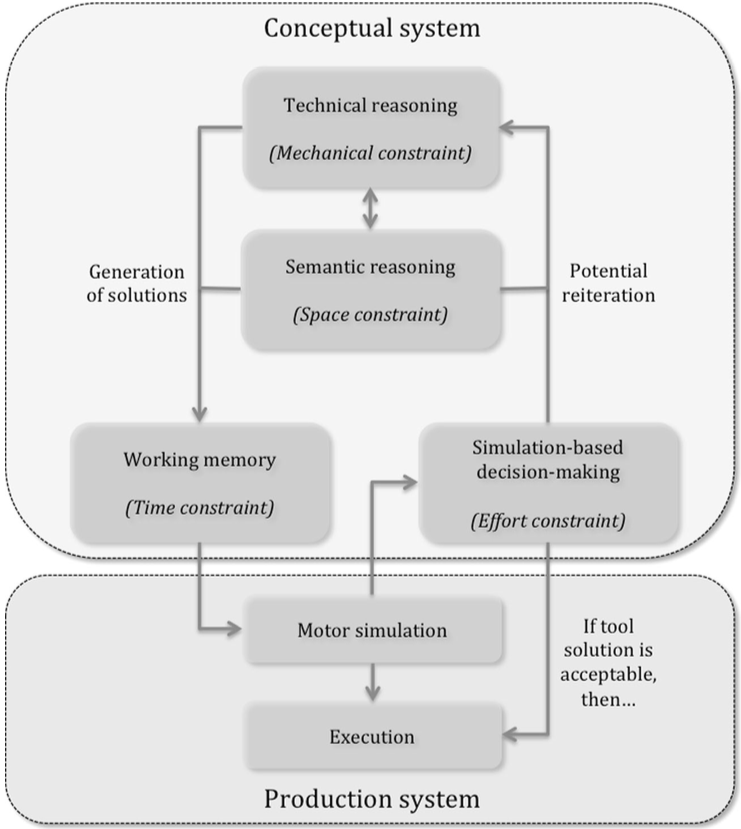
\includegraphics[width=.9\textwidth]{figures/4CTArchitecture.png}
  \caption{4CT architecture reprinted from \cite{osiurak2014a}}
  \label{fig:4CTArchitecture}
\end{figure}      

Unlike competing theories, 4CT distinguishes between conceptual and production systems when describing tool use (fig. \ref{fig:4CTArchitecture}).
The production system dictates movement by transforming a person's intent into motor control while the conceptual system encapsulates the cognitive reasoning necessary for tool use.
The dissertation focused on a computational model for the latter.


%-----------
% More paragraphs needed to explain why 4CT is desired over other theories ?
%-----------

4CT characterises tool use situations as problem solving tasks requiring strong cognitive abilities. 
The four constraints of mechanics, space, time, and effort are dimensions within which problems are defined.
Aiding problem solving are four cognitive processes: technical reasoning, semantic reasoning, working memory, and simulation based decision making (fig. \ref{fig:4CTArchitecture}).  
Even a simple scenario like slicing bread is a reasoning task about the knife's length, sharpness, serration and the movements necessary to manifest cutting effects. 

Problem solving becomes more apparent in the absence of familiar tools, when subjects have to repurpose tools or fashion new ones.
A distinction is made between novel tool use and familiar tool use. 
Semantic reasoning refers to situations when subjects are accustomed to a tool's common purpose. 
For example, a serrated knife can be used for cutting bread. 
These associations are made on prior experience without considering the knife's physical properties.  
In novel cases, however, technical reasoning is the inference of how the tool's properties can solve problems.
For example, in the absence of a bread knife a saw would be a better cutting device than a table knife. 
Technical reasoning is a more general process for solving problems, although more cognitively involved.  

The effort constraint and simulation based decision making refer to tool use energy cost. 
In nature, a simple rule of survival is that actions should require less energy than the rewards gained \cite{proffitt2006}.
Perceived effort would explain a user's preference for one tool use method over another. 
Even with multiple tools available, differences in physical properties can lead to differences in effort and dictate choices made. 

The working memory process (fig. \ref{fig:4CTArchitecture}) is required when multiple steps must be fulfilled to achieve a goal. 
It describes a subject's ability to split activities into sub-goals and hold them in memory. 
Complex tasks such as fixing a broken radio would involve multiple steps and tool selection, however, such complex objectives are beyond the scope of this project.

A computational model should initially solve simple tool-use problems before complex ones.
Our focus is therefore on single step tool and object interaction involving generic situations.
These situations would be best solved through technical reasoning due to its general problem solving abilities. 
However, 4CT does not explain more complex reasoning than about simple object properties such as length, sharpness, abrasiveness.
Crucial factors of forces and geometric constraints are simply abstracted as mechanical knowledge. 
A computational model would therefore have to elaborate these items before fitting into the larger 4CT framework. 

The topic of this paper is solving geometric constraints through spatial reasoning in order to achieve simple tool-object interaction.  

\subsection{Experimental Setup}

Dietmar Heinke and Fran\c{c}ois Osiurak,the author of 4CT, have devised an experiment that tests human ability to use novel objects. 
The experiment is intended for use in both a computational model and to investigate human reasoning on tool and object geometries. 
Human trials were run in parallel to this project but do not constitute part of it. 
Nevertheless, this paper will refer to behaviour observed in these trials even though data has not yet been published. 

\begin{figure}[!h]
  \centering
  \begin{subfigure}{0.49\textwidth}
    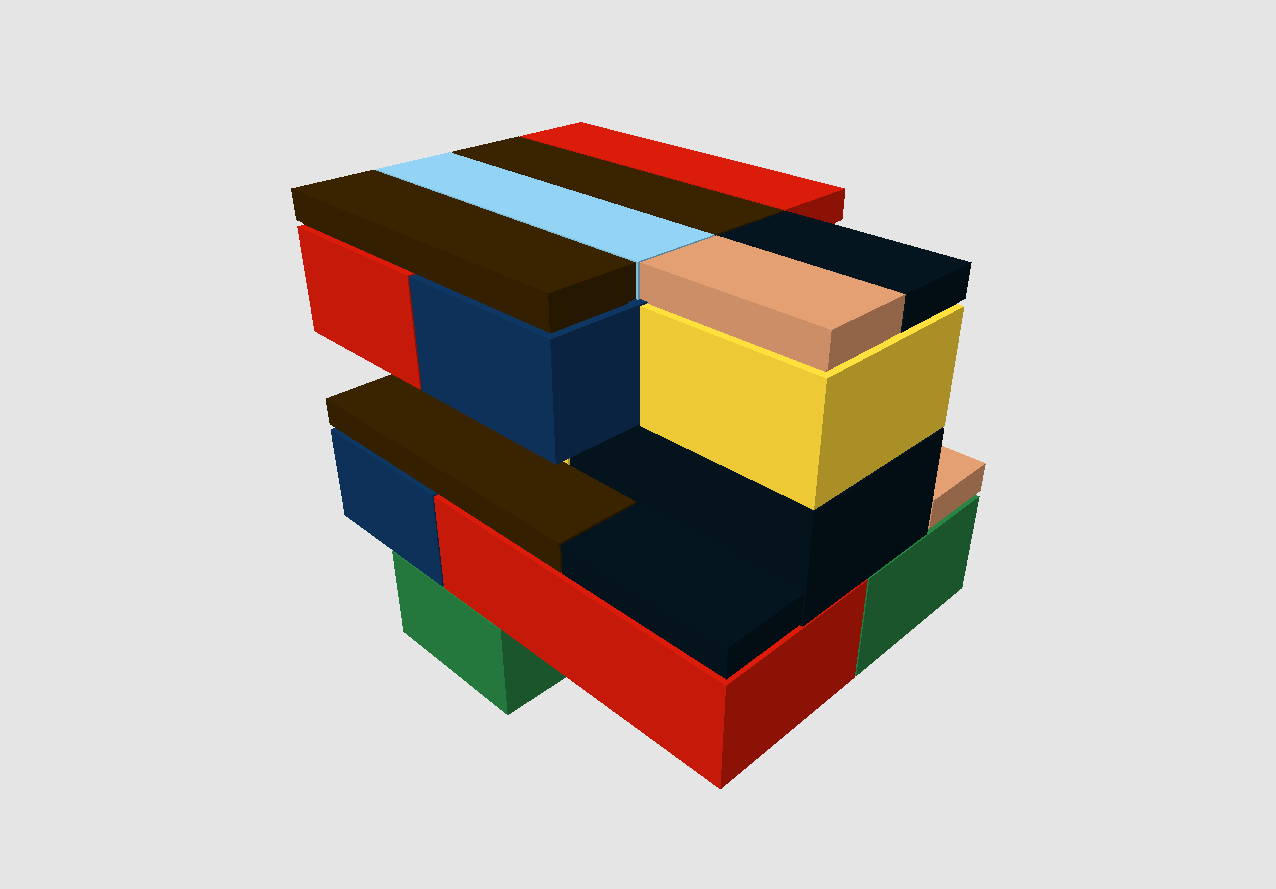
\includegraphics[width=1\linewidth]{figures/obj51.png}
    \caption{Passive object}
    \label{fig:obj51}
  \end{subfigure}
  \begin{subfigure}{0.49\textwidth}
    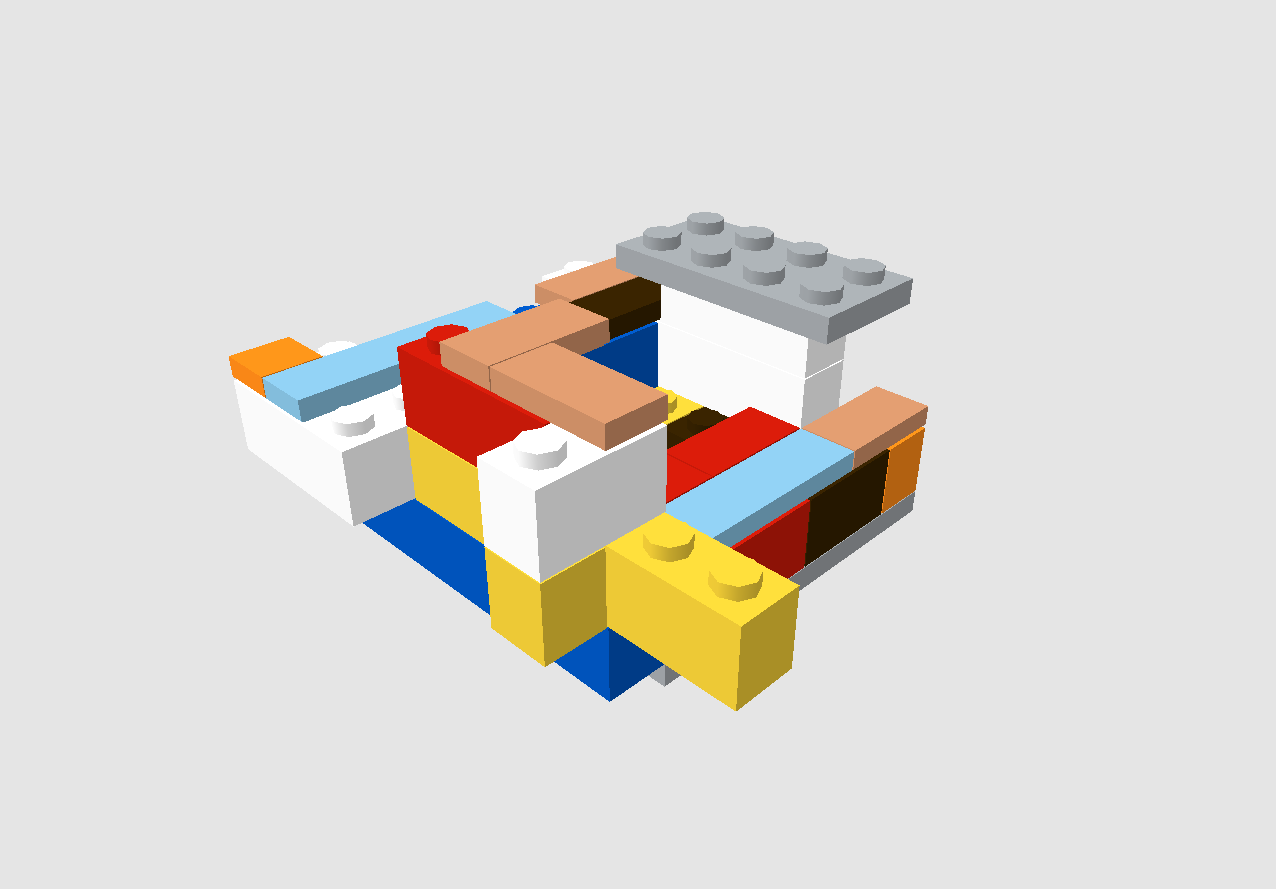
\includegraphics[width=1\linewidth]{figures/obj52.png}
    \caption{Active object}
    \label{fig:obj52}
  \end{subfigure}
  \caption{Pair of novel tool and object models}
\end{figure}

In the experiment a subject is presented two novel objects built with LEGO blocks.
One item is introduced to participants as "passive object" and may not be directly touched (fig. \ref{fig:obj51}).
The second item is introduced as an " active object" and must be used to lift the passive object to a new location (fig. \ref{fig:obj52}).
Note that the active and passive objects are analogous to tool and target objects respectively.
Due to the unusual geometries, participants must reason about how to complementary match the tool and object shapes.

A computational model mimicking human behaviour, would solve geometric constraints similarly to human subjects.
Formally solving the experimental task requires consideration of force closure - object motion is controlled by tool contact forces.
To shortcut the computing of forces and physical interaction one can use a physics engine. 
To some extent, it is believed that the human brain computes approximate Newtonian laws \cite{battaglia2013}. 
Similarly to humans, a physics engine does not compute exact friction, closure or gravitational forces, but provides realistic approximate results. 
A tool use model can employ physics engines for  multiple reasons:
\begin{enumerate}
\itemsep0em 
\item The engine can serve as a source of inference over physical laws and objects 
\item Solutions of tool-object interactions can be verified through simulation
\item Physical simulation is analogous to mental tool simulation from 4CT
\end{enumerate}

\subsection{Physics Engine Evaluation}

A suitable physics engine would satisfy the following criteria:
\begin{enumerate}
\item The engine should have high fidelity in simulating rigid body collision. 
That is, the engine should faithfully reflect real world interaction of bodies involving no moving parts or deformations.
As tool and object are composed of LEGO, items are best represented as rigid bodies.   
High fidelity is required to find realistic tool-object fitting positions, with minimal errors.
\item The engine should be available in user-friendly scientific languages (such as MATLAB or Python). 
Scientific languages have inbuilt algorithms that can be utilised.
\item Engine use should be inexpensive.
\item The engine should be portable to common platforms (i.e. Windows, Linux, MacOS) to encourage engagement from future researchers.
\item The engine should have good documentation for ease of development.
\item Simulations must be done on three dimensional(3D) models of tools and objects.
Engines capable of only two dimensional(2D) simulations are therefore inappropriate.  
\end{enumerate}

In an academic context, physics engines have been used for robotic simulation of locomotion and object grasping.
The fidelity of these scenarios match our experimental requirements and can serve as a basis for engine evaluation. 
Literature reviews have focused on commercial or open source engines dedicated to game development \cite{boeing2007,roennau2013,hummel2012}. 
Engines aimed at scientific simulation unfortunately require large usage fees (e.g. Vortex by CM-Labs and MuJoCo).
Due to their target audience, game engines achieve high speed simulations at the cost of precision. 
There is compromise between speed and how faithfully an engine can replicate real physical interaction.
For this reason, most available engines are not suitable for scientific use. 

With engines undergoing constant improvement, evaluation is transient and specific to product versions. 
Review articles fail to specify the version of the engines evaluated.
Additionally, performance results are influenced by implementation specifics.
For example, reviewers can use the engine directly or through an abstraction layer that can affect performance.  
We therefore select the most likely engines for model use, and evaluate individually. 

Two game engines emerged as candidates: \emph{Bullet Physics v2} and \emph{Newton Game Dynamics v3}.
A formerly popular option is Open Dynamics Engine, but should not be considered as it is no longer under active development. 

\subsubsection{Bullet Physics}
\cite{boeing2007} regards Bullet as having the best overall performance. 
\cite{hummel2012,roennau2013} also mention Bullet as having the best rigid body collision, but only in the case of large object simulation.
What defines objects as large is however unclear. 

\begin{figure}[h]
  \centering
  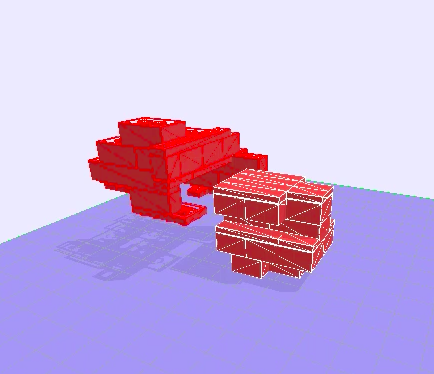
\includegraphics[width=.5\textwidth]{figures/bullet_demo.png}
  \caption{Tool and object models loaded into Bullet simulation demo}
  \label{fig:bullet_demo}
\end{figure}      

We test Bullet's collision detection in a demo containing simple tool and object models (fig. \ref{fig:bullet_demo}).
The passive object is first set on a flat surface.
The tool is then positioned to slide into the object and lift it.
Demo code is therefore representative of the experimental setup.  

Several parameters can influence the effects of interaction between the two objects:
\begin{enumerate}
\item Object collision properties are more commonly represented by classes which approximate the object's shape in order to gain execution speed.
A more precise approach is to use classes that represent true shape properties(fig. \ref{fig:collision_shape}).   

\begin{figure}[h]
\centering
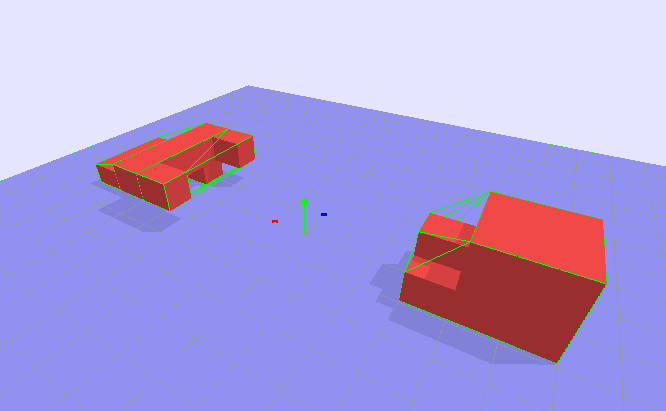
\includegraphics[width=.48\textwidth]{figures/collision_approximation.png}
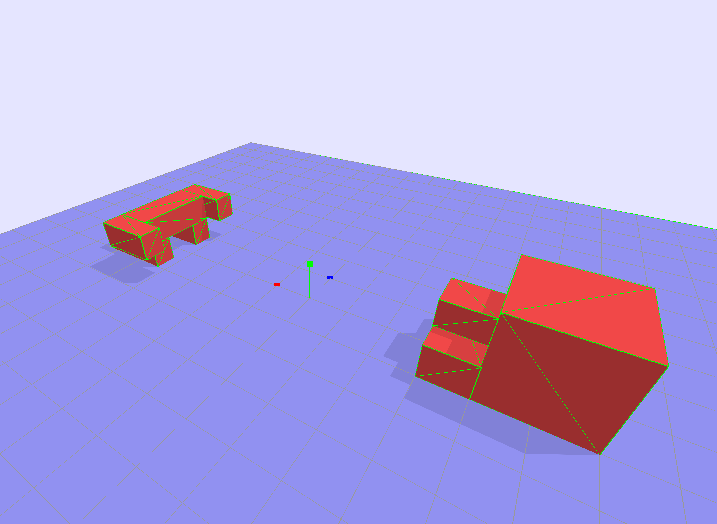
\includegraphics[width=.41\textwidth]{figures/collision_exact.png}
\caption{Comparison of approximated collision and exact collision shape represented as green lines}
\label{fig:collision_shape}
\end{figure}      

\item A threshold or margin of contact exists between objects. 
When the margin is low, shaking effects can be noticed when objects make contact. 
Alternatively, when the margin is large, the object's collision would not be representative as gaps would be too small to allow fitting. 

\item Moving the tool to interact with the object can be done multiple ways with variable degrees of realism.
\end{enumerate}

From a development perspective, the engine is easy to compile and has detailed documentation.
MATLAB integration is available from third party developers, but is not well maintained, lacking functionality or failing compilation.
A model using Bullet Physics would therefore have to be developed in C++. 

Overall \emph{Bullet Physics} suffers from a high degree of shaking when tool and object interact. 
When the tool is positioned to lift the object, collision points make the object bounce uncontrollably within the tool's grasp. 
As bounce forces amplify the object eventually bursts out of the tool's fixation.  
Engine parameters can be tuned to minimise these effects, but would ultimately lead to less representative simulations. 

\subsubsection{Newton Game Dynamics}
Newton Game Dynamics is regarded as having better precision than Bullet, but at the cost of performance \cite{hummel2012}. 
The precision gain is achieved by using a deterministic solver instead of numerical methods for integrating movement and forces over time. 

\begin{figure}[h]
  \centering
  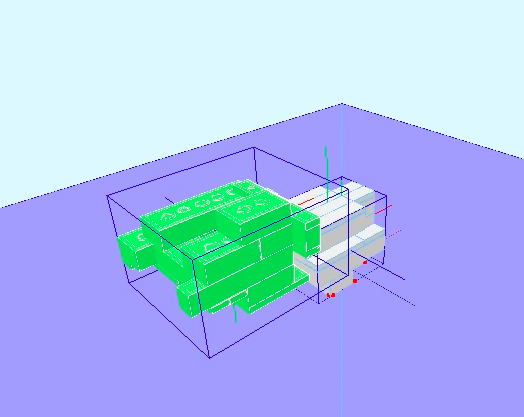
\includegraphics[width=.5\textwidth]{figures/newton_demo.png}
  \caption{Tool and object models loaded into Bullet simulation demo}
  \label{fig:newton_demo}
\end{figure}      

We setup a demo similar to Bullet.
The object is set on a flat surface. 
The tool is then slid into the object's fitting and lifted (\ref{fig:newton_demo}). 

Compared to Bullet, Newton's default behaviour exhibits realistic behaviour. 
The simulation shows no shaking or unrealistic dynamics.
The tool and object move smoothly on established trajectories. 

From a development point of view, Newton lacks the quality of documentation found in Bullet. 
There are thousands of lines of sample code available, but locating needed functionality is difficult. 
This is made worse by a strange, yet consistent API interaction.

Additionally, the engine supports unconventional 3D file formats, making it difficult to load object models.
Code has to be developed to support common formats.

As a less popular engine, Newton does not have integration with other languages (e.g. MATLAB or Python). 
A computational model would have to be written in C++.

Even with the above development concerns, the engine's simulation precision make it a prime candidate for our model.  

\section{Exhaustive Search}
Demos show how tool use can be verified through simulation.
As the model aims to solve geometric constraints, one can position items in all possible configurations and select valid ones. 
Validity implies that the tool can lift the object, and that models do not penetrate each other's surfaces.
A single configuration represents a tool's rotation and relative position to the object.
That is X,Y,Z coordinates and rotations around axes (i.e. yaw, pitch, roll). 
The \emph{Exhaustive Search} model finds solutions by testing all possible configurations.

\subsection{Implementation}
The target object is positioned on a flat surface. 
The tool is then placed in successive relative locations, and object collision is tested. 
For any collision points to be detected, one physics simulation time step has to be executed.
Newton Physics allows obtaining the penetration depth of collision points. 
When penetration is too high, the configuration is deemed invalid as objects unrealistically penetrate each other's bodies.

If penetration depth is zero, the object and tool may not be in contact at all. 
Such scenarios can be removed by applying a lifting force to the tool.
When the objects are in contact, lifting velocity would transfer to the target object and can be asserted. 

The approach is able to verify a fitting configuration for a single physics engine update step.
However, as object contact is detected through a small penetration margin it is possible that undesired vertical forces appear.
Output data may therefore contain invalid solutions which require further validation.

The physics engine does not require 3D rendering when computing interaction. 
Exhaustive searching can run in either graphical or non-graphical modes.
Graphical rendering allows researchers to investigate the correct loading of objects and 3D world dynamics.
The non-graphical model allows faster computation as rendering overburden is removed. 

\begin{figure}[h]
  \centering
  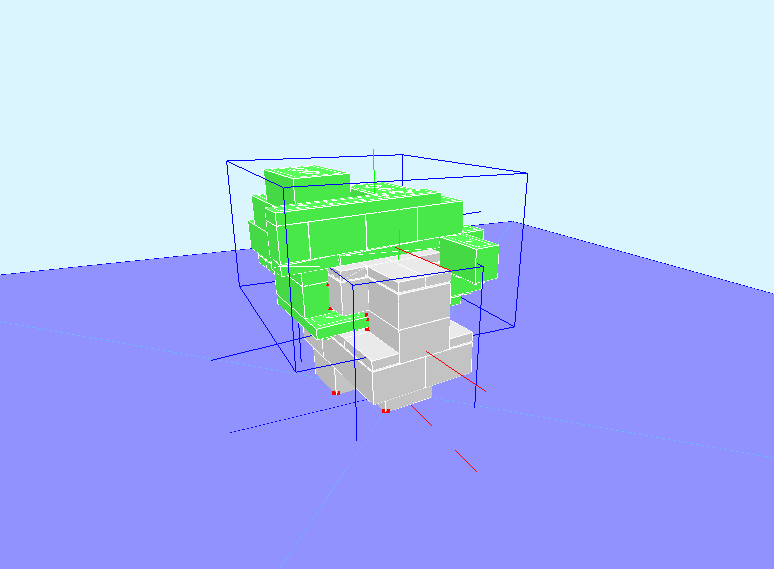
\includegraphics[width=.7\textwidth]{figures/newton_simulation.png}
  \caption{Exhaustive search rendering}
  \label{fig:newton_simulation}
\end{figure}      

Figure \ref{fig:newton_simulation} captures the rendering of two objects in fitting position.
Object bodies are displayed in green and grey.
Collision meshes are outlined by white lines.
Contact points are displayed as red dots.
3D orientation vectors give visual cues of rotation angles (red, green, blue for X, Y, Z respectively).
Blue bounding boxes represent vertex extremities (i.e. min and max X, Y, Z coordinates).
 
Newton Dynamics has the in built ability to optimise meshes as convex decomposition.
This means, complex assemblies of triangles representing simple geometries can be optimised to simpler mesh structures of the same shapes. 
A complex object would therefore be transformed to an assembly of simple shapes, optimising collision detection and computation. 
This feature may occasionally have to be tuned for pairs of tool-object models.

\subsection{Discussion}
When search intervals are in the vicinity of possible solutions, the model finds multiple equivalent fitting configurations.
Equivalent solutions are found on the trajectory on which the tool slides into the object.
However, on a single multi-core computer exhaustive searching is  not feasible. 
The tool's position is determined by 6 degrees of freedom amounting to $~10^{12}$ possible configurations. 
Even for a single tool rotation there are $~10^8$ configurations, requiring approximately an hour of execution. 

In the implementation verifying configurations has been optimised for speed.
Further improvements can be achieved by splitting the search space over multiple computers.
Alternatively, the search step can be increased at the expense of finding possible solutions. 

Exhaustively searching is lengthy and computationally expensive.
Engine features, such as penetration depth, can be utilised in more ingenious search algorithms.
However, solutions based solely on the engine's functionality remain problematically unrealistic representations of physical laws and human ability.
For example, the tool can be positioned to lift an object even when no physical manner would allow it to be placed in that location.  


In simulations lifting forces are applied to the tool's center of gravity.
This is a strong simplification of the problem as the search may produce solutions that do not realistically permit the tool to be held.

Computational expense remains the impeding factor to the model's use. 
Heuristic methods can be used to optimise the search space whilst considering human ability.
The following describes a visual search approach to finding possible fitting configurations. 
The physics simulations remain a method for testing such configurations. 

%\printbibliography

\end{document}
